\documentclass[tikz]{standalone}
\usepackage{pgfplots}
\pgfplotsset{compat=1.15}
\usepackage{mathrsfs}
\usetikzlibrary{arrows,calc}
\usepackage{tkz-euclide}

\pagestyle{empty}

\definecolor{AngleClr}{rgb}{0,0.39215686274509803,0}
\definecolor{ShapeClr}{rgb}{0.6,0.2,0}

\begin{document}

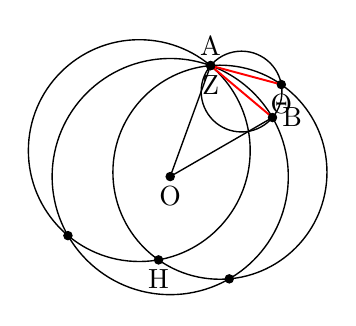
\begin{tikzpicture}[scale=.75]
\tkzSetUpLine[line width=1pt,color=black]
\tkzSetUpPoint[fill=black]

\tkzDefPoints{0/0/O,2/0/X}

\tkzDefPoint(70:2){A}
\tkzDefPoint(30:2){B}

\tkzDefPoint(-150:2){C}
\tkzDefPoint(-60:2){D}

\tkzDefMidPoint(A,B) \tkzGetPoint{MB}
\tkzDefMidPoint(A,C) \tkzGetPoint{MC}
\tkzDefMidPoint(A,D) \tkzGetPoint{MD}

\tkzInterCC(MB,B)(MC,C) \tkzGetPoints{X}{Z}
\tkzInterCC(MC,C)(MD,D) \tkzGetPoints{X}{H}
\tkzInterCC(MD,D)(MB,B) \tkzGetPoints{X}{Th}


\tkzDrawCircle[color=black,line width=0.5pt](O,X)
\tkzDrawCircles[color=black,line width=0.5pt](MD,D MB,B  MC,C)
\tkzDrawSegments[line width=0.5pt,color=black](O,A O,B)
\tkzDrawSegments[line width=0.7pt,color=red](A,B Z,Th)

\tkzDrawPoints[size=3](A,B,O,C,D,Z,H,Th)
\tkzLabelPoint[above](A){$\rm A$}
\tkzLabelPoint[right](B){$\rm B$}
\tkzLabelPoint[below](O){$\rm O$}

\tkzLabelPoint[below](Z){$\rm Z$}
\tkzLabelPoint[below](H){$\rm H$}
\tkzLabelPoint[below](Th){$\rm \Theta$}

\end{tikzpicture}
\end{document}
